{

\pagestyle{fancy}

\pagestyle{fancy}
\fancyhead{}


\hypersetup{linkcolor=black}

\lhead{Table des matières}

% Table of contents -------------------------------------------------
\tableofcontents\thispagestyle{fancy}
\listoffigures
\listoftables

% Chapter 1 Introduction ---------------------------------------------------------
% -------------------------------------------------------------------
\pagebreak
\lhead{Introduction}
\chapter{Introduction}\thispagestyle{fancy}


\section{Présentation du projet}
It contains sophisticated software tools and components with which you can construct (typeset) a wide range of documents. The sub-title of this article also poses two questions about .

\subsection{Idée initiale}
h you can construct (typeset) a wide range of documents. The sub-title of this art

\subsection{Solution de la problematique}
h you can construct (typeset) a wide range of documents. The sub-title of this art


\section{Etat de l'art}

\subsection{Les services offertes}
h you can construct (typeset) a wide range of documents. The sub-title of this art

\subsection{Comparison avec autres produits}
h you can construct (typeset) a wide range of documents. The sub-title of this art

% Chapter 2 Raspberry PI ---------------------------------------------------------
% -------------------------------------------------------------------

\pagebreak
\lhead{Raspberry PI}

\chapter{Raspberry PI}\thispagestyle{fancy} % ----------

\section{Module PI3}

\section{Autres composantes}
    \subsection{Caméra}
    \subsection{Button}
    \subsection{Antenne WI-FI}
    \subsection{Bloque d'alimentation}

\section{Schéma de montage}
    

% Chapter 3 Deep learning ---------------------------------------------------------
% -------------------------------------------------------------------

\pagebreak
\lhead{Deep learning}

\chapter{Deep learning}\thispagestyle{fancy}
\section{Facial recognition}
\subsection{Dataset}

\subsection{LBH}
development for over 10 years
\subsubsection{Training LBH}
\subsubsection{Testing LBH}

\subsection{CNN}
\subsubsection{Training CNN}
\subsubsection{Testing CNN}
\section{Tesseract OCR}
\subsubsection{Testing Tesseract}
\section{YOLOv4}
\subsection{Training YOLOv4}
\subsubsection{3-classes}
\subsubsection{11-classes}
\subsubsection{80-classes}
\subsection{Testing YOLOv4}


% Chapter 4 Version I ---------------------------------------------------------
% -------------------------------------------------------------------

\pagebreak
\lhead{Version I : Traitement image}

\chapter{Version I : Traitement image}\thispagestyle{fancy}

\section{API}

    \subsection{Définition}
En informatique, une \textbf{API} (application programming interface) ou interface de programmation applicative est un ensemble normalisé de classes, de méthodes, de fonctions et de constantes qui sert de façade par laquelle un logiciel offre des services à d'autres logiciels. Elle est offerte par une bibliothèque logicielle ou un service web, le plus souvent accompagnée d'une description qui spécifie comment des programmes consommateurs peuvent se servir des fonctionnalités du programme fournisseur.\\[0.5cm]

De manière plus générale, on parle d'\textbf{API} à partir du moment où une entité informatique cherche à agir avec ou sur un système tiers, et que cette interaction se fait de manière normalisée en respectant les contraintes d'accès définies par le système tiers. On dit que le système tiers « expose une \textbf{API}». À ce titre, des choses aussi diverses que la signature d'une fonction, une \textbf{URL} … sont parfois considérés comme des API (ou \textbf{micro-API}) à part entière.\\[0.5cm]

% include {float} package and add [h] to prevent putting the figure in the end of the chapter
\begin{figure}[h] 
\centering
\frame{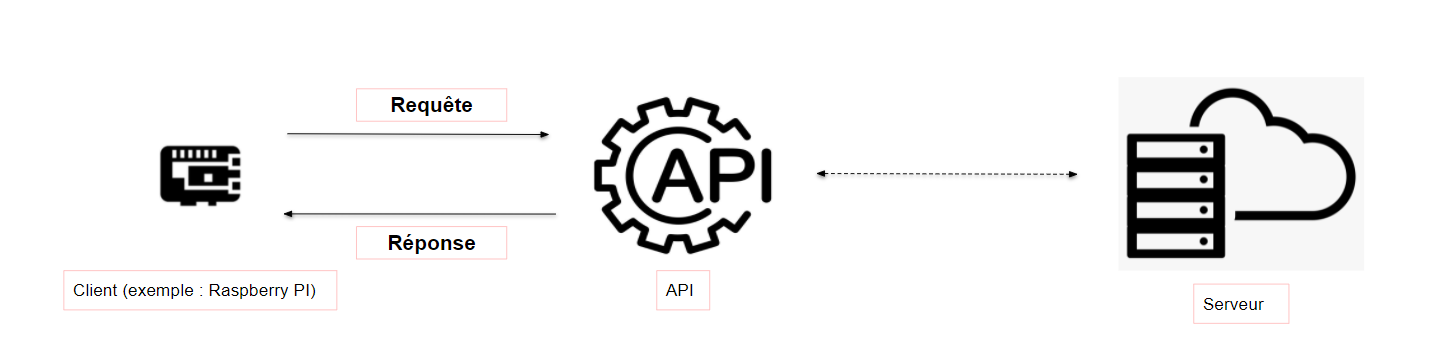
\includegraphics[width=17cm, height=5cm]{3-Figures/client-server-archi.PNG}}\\[0.5cm]
\caption{API}
\label{fig:figure2}
\end{figure}

L'image ci-dessus montre l'architecture client-serveur où l'on voit clairement l'API entre le serveur et le client. Le client envoie une requête à l'API pour demander des services au serveur, ce dernier transmettra la requête au serveur afin qu'il renvoie la réponse au client.

    \subsection{RestAPI}
Il y a un type d'API qui s'appele \textbf{REST API} (\textbf{Representational State Transfer Application Program Interface}) est un style architectural qui permet aux logiciels de communiquer entre eux sur un réseau ou sur un même appareil. Le plus souvent les développeurs utilisent des API REST pour créer des services web. Souvent appelés services web RESTful, REST utilise des méthodes HTTP pour récupérer et publier des données entre un périphérique client et un serveur.

Le concept fondamental de toute \textbf{REST API} est la ressource. Une ressource est un objet avec un type, des données associées, des relations avec d'autres ressources et un ensemble de méthodes qui fonctionnent dessus.

En rapport avec notre project, les ressources qu'on possède sont les trois services suivantes : Prédiction visage, prédiction de texte et prédiction d'objets.\\[0.5cm]

\begin{figure}[h] 
\centering
\frame{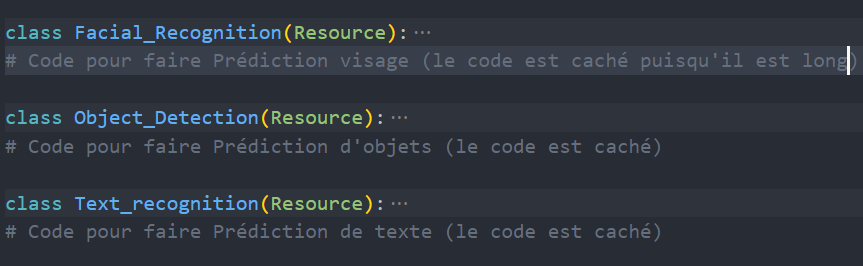
\includegraphics[width=17cm, height=5cm]{3-Figures/resources.PNG}}
\caption{Ressources d'API}
\label{fig:figure2}
\end{figure}
Chaque ressource est définie par une URL dont la première partie est l'adresse IP du serveur et la deuxième est un chemin spécifique qui commence par "/" comme le montre l'image en dessous.

\begin{figure}[h] 
\centering
\frame{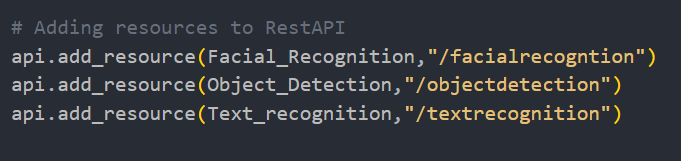
\includegraphics[width=13cm, height=3cm]{3-Figures/add-resources.PNG}}
\caption{Ajout des ressources}
\label{fig:figure2}
\end{figure}

Donc on a ajouté les ressources à notre variable \textbf{api} en spécifiant les chemins pour distinguer entre les 3 ressources. Si par exemple le client veut bénéficier du premier service et que le serveur a l'adresse ip suivante \textbf{\textcolor{blue}{10.1.1.18}}, le client enverra une requête HTTP à \textbf{\textcolor{blue}{'http://10.1.1.18/facialrecognition'}} contenant une image et il recevra en retour le résultat de la prédiction. Tout cela est du côté serveur, nous montrerons ensuite ce qui se passe du côté client

    \subsection{Test avec Postman}

Postman est une application utilisée pour les tests d'API. Il s'agit d'un client HTTP qui teste les requêtes HTTP, en utilisant une interface utilisateur graphique, à travers laquelle nous obtenons différents types de réponses qui doivent ensuite être validées
\begin{figure}[h] 
\centering
\frame{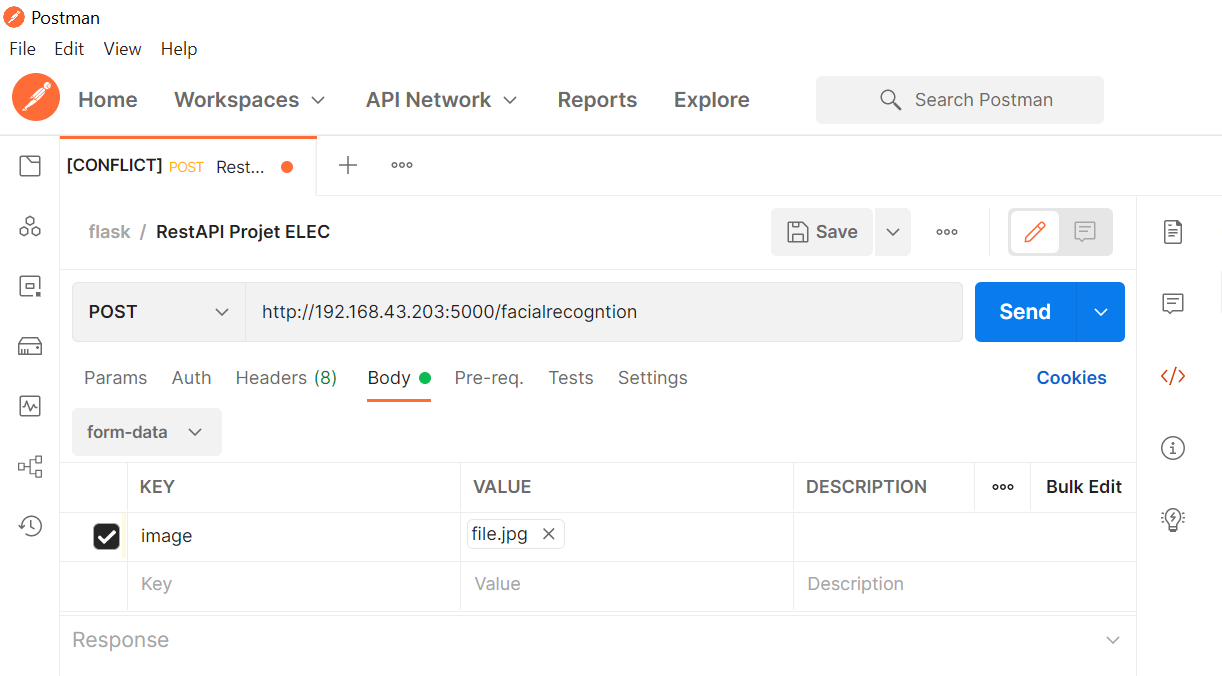
\includegraphics[width=13cm, height=7cm]{3-Figures/postman.PNG}}
\caption{Postman}
\label{fig:figure2}
\end{figure}

Nous spécifions le chemin pour envoyer la requête HTTP and choose one image to send.



\section{Code en locale}
\subsection{http request}
\subsection{Texte-audio}



% Chapter 5 Traitement video ---------------------------------------------------------
% -------------------------------------------------------------------
\pagebreak

\lhead{Version II : Traitement video}
\chapter{Version II : Traitement video}\thispagestyle{fancy}


\section{Sockets}
In terms, “the new kid on the block” despite having been in active development for over 10 years.

\section{Modèles Deep learning}
In terms, “the new kid on the block” despite having been in active development for over 10 years.
\subsection{LBH}
\subsection{Handwritting recognition}
\subsection{YOLOv4 80 classes}


% Chapter 4 ---------------------------------------------------------
% -------------------------------------------------------------------

\pagebreak
\lhead{Démonstration}
\chapter{Démonstration}\thispagestyle{fancy}

% Chapter 5 ---------------------------------------------------------
% -------------------------------------------------------------------

\pagebreak
\lhead{Organisation}

\chapter{Organisation}\thispagestyle{fancy}
\section{Gantt}
A Gantt chart is a type of bar chart that illustrates a project schedule, named after its popularizer, Henry Gantt, who designed such a chart around the years 1910–1915. Modern Gantt charts also show the dependency relationships between activities and the current schedule status

\section{Github}
GitHub, Inc. is a provider of Internet hosting for software development and version control using Git. It offers the distributed version control and source code management functionality of Git, plus its own features

\section{Budget}
GitHub, Inc. is a provider of Internet hosting for software development and version control using Git. It offers the distributed version control and source code management functionality of Git, plus its own features

% Chapter 6 ---------------------------------------------------------
% -------------------------------------------------------------------


\pagebreak
\lhead{Code source du projet}
\chapter{Code source du projet}\thispagestyle{fancy}
Vous trouvez dans ce \href{https://github.com/mohammedAljadd/iEars}{lien} le code source de notre projet inclu les deux versions.\\

\begin{center}
\begin{figure}[h]
\centering
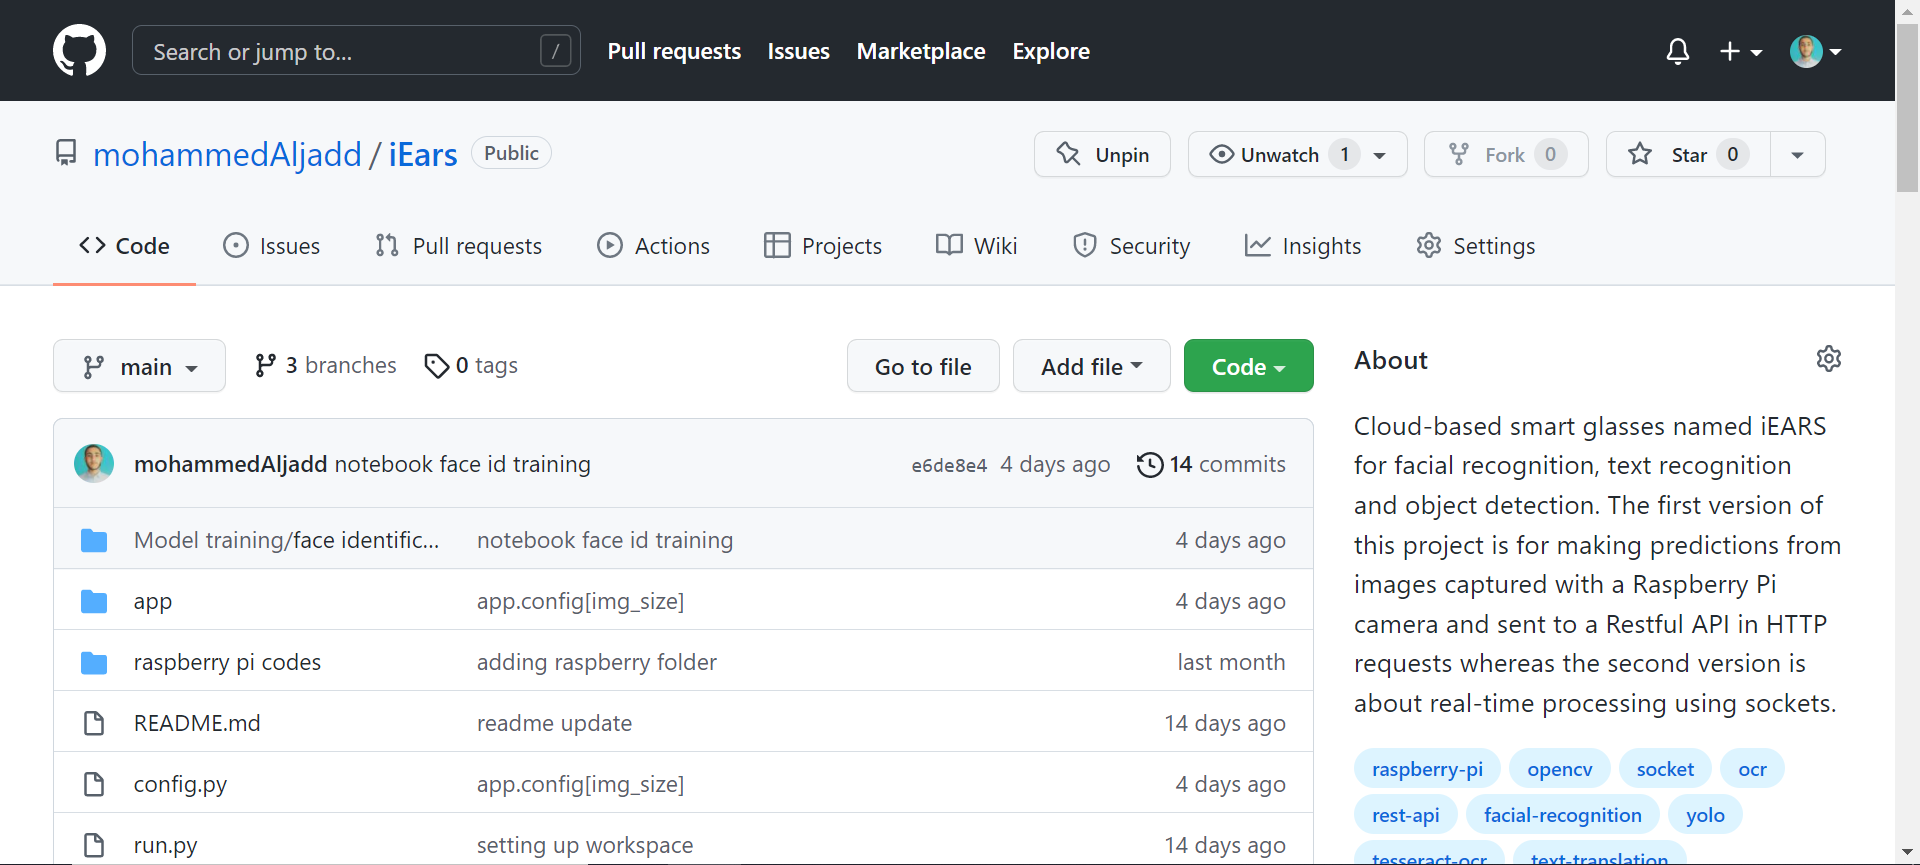
\includegraphics[width=18cm, height=9cm]{4-Images/github.PNG}\\[2cm]
\caption{Github}
\label{fig:figure2}
\end{figure}
\Large

\end{center}

% Chapter 7 ---------------------------------------------------------
% -------------------------------------------------------------------

\pagebreak
\lhead{Bibliographie}
\chapter*{Bibliographie}
\printbibliography 

}